\section{Forward Security}
\label{sec:forward-sec}

\paragraph{Motivation} Until now, we have used a secret key that was only known by one or more honest parties participating in the various protocols.
However in the real world, the secret key often gets compromised, and the adversary learns some information about it.
This might happen if the device gets stolen or confiscated, if the honest parties get hacked or just through human error.
If we use our KEM from Figure~\ref{fig:kem:const:elgamal} as an example, this would enable the adversary to decapsulate every single ciphertext that was sent (if the adversary recorded the ciphertexts).
Forward Security guarantees that messages before the compromise remain secure (Figure~\ref{fig:fs:sketch}).

In this section, we will discuss how to achieve security even if the secret key is compromised in the future, using our KEM as an example.

\begin{figure}[!ht]
    \centering
    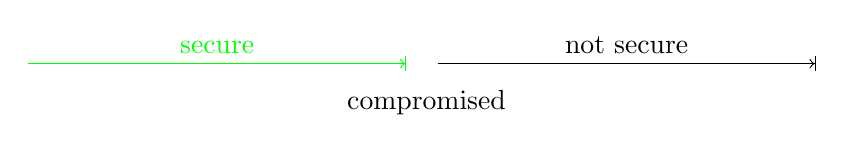
\begin{tikzpicture}%
    \draw [green, -{>Bar}] (0,0) -- (4.8,0) node [midway, above] {secure};
    \node at (5,0) {\color{red}\LARGE\Lightning};
    \node at (5,-.5) {$\dk$ compromised};
    \draw [-{>Bar}] (5.2,0) -- (10,0) node [midway, above] {not secure};
\end{tikzpicture}%
    \caption{A sketch of forward security}
    \label{fig:fs:sketch}
\end{figure}

\subsection{Forward Secure KEMs}

\alert{add \cite{SP:GreMie15,EC:CanHalKat03,EC:GHJL17}}

\paragraph{Syntax} To provide security even if the secret key is leaked, we have to change the secret key over time.
This means we also need to change the syntax of the decapsulation algorithm.
The forward-secure KEM $\FKEM=(\FKEMgen,\FKEMenc,\FKEMdec)$ is a tuple of three algorithms with encapsulation key space~$\eksp$, decapsulation key space~$\dksp$, ciphertext space~$\csp$, and symmetric key space~$\ksp$:
\begin{itemize}
    \item $\KEMgen: \emptyset \tor \dksp\times\eksp$
    \item $\KEMenc: \eksp \tor \ksp\times\csp$
    \item $\KEMdec: \dksp\times\csp \to \dksp\times\ksp$
\end{itemize}

\paragraph{Correctness} A forward-secure KEM $\FKEM$ is correct if $\Pr[\CORR_{\FKEM}(\advA)=0]=1$ for all adversaries~$\advA$, where game~$\CORR$ is defined in Figure~\ref{fig:fkem:corr}.

\paragraph{Security}
The advantage of an adversary~$\advA$ against forward-secure KEM $\FKEM$ in game $\INDCCA$ from Figure~\ref{fig:fkem:ind} is defined as:
\[
\Adv_\FKEM^\indcca(\advA)\coloneqq\left|\Pr[\INDCCA_{\FKEM}^0(\advA)=1]-\Pr[\INDCCA_{\FKEM}^1(\advA)=1]\right|\text{.}
\]

\begin{figure}[!ht]
    \begin{subfigure}{.49\textwidth}
        \centering
        \nicoresetlinenr%
        \fbox{%
            \scalebox{\codescalefactor}{%
                % !TeX root = ..\..\main.tex
\markersetlen{ndL}{120pt}%
\markersetlen{ndR}{130pt}%
\newcommand{\CK}{\mathit{CK}}%
\begin{tabular}[t]{ll}
    \nicodemusbox{\markerlenndL}{%
        \textbf{Game} $\CORR_{\FKEM}(\advA)$
        \begin{nicodemus}
            \item $\CK[\cdot]\gets\bot$
            \item $(\dk,\ek)\getsr\FKEMgen$
            \item Invoke $\advA(\ek)$
            \item Stop with~$0$
        \end{nicodemus}%
        \medskip
        
        \textbf{Oracle} $\Oenc$
        \begin{nicodemus}
            \item $(k,c)\getsr\FKEMenc(\ek)$
            \item If $\CK[c]\neq\diamond$: $\CK[c]\gets k$
            \item Return~$c$
        \end{nicodemus}%
    }%
    &
    \nicodemusbox{\markerlenndR}{%
        \textbf{Oracle} $\Odec(c)$
        \begin{nicodemus}
            \item $(\dk,k')\gets\FKEMdec(\dk,c)$
            \item If $\CK[c]\notin\{k',\bot,\diamond\}$:
            \item \quad Stop with $1$
            \item If $\CK[c]\neq\bot$: $\CK[c]\gets \diamond$
            \item Return $k'$
        \end{nicodemus}%
    }%
\end{tabular}%%
            }%
        }
        \caption{%
            $\CORR$ game.
        }
        \label{fig:fkem:corr}    
    \end{subfigure}
    \hfill
    \begin{subfigure}{.49\textwidth}
        \centering
        \nicoresetlinenr%
        \fbox{%
            \scalebox{\codescalefactor}{%
                % !TeX root = ..\..\main.tex
\markersetlen{ndL}{130pt}%
\markersetlen{ndR}{130pt}%
\newcommand{\CC}{\mathit{CC}}%
\begin{tabular}[t]{ll}
    \nicodemusbox{\markerlenndL}{%
        \textbf{Game} $\INDCCA_{\FKEM}^b(\advA)$
        \begin{nicodemus}
            \item $x\gets 0$
            \item $\CC\gets\emptyset$
            \item $(\dk,\ek)\getsr\FKEMgen$
            \item $b'\getsr\advA(\ek)$
            \item Stop with~$b'$
        \end{nicodemus}%
        \medskip
        
        \textbf{Oracle} $\Ochall$
        \begin{nicodemus}
            \item If $x=1$: Return $\bot$
            \item $(k_0,c)\getsr\FKEMenc(\ek)$
            \item $k_1\getsr\ksp$
            \item $\CC\gets\CC\cup\{c\}$
            \item Return~$(k_b,c)$
        \end{nicodemus}%
    }%
    &
    \nicodemusbox{\markerlenndR}{%
        \textbf{Oracle} $\Odec(c)$
        \begin{nicodemus}
            \item $(\dk,k)\gets\FKEMdec(\dk,c)$
            \item If $c\in\CC$: $k\gets\bot$
            \item $\CC\gets\CC\setminus\{c\}$
            \item Return $k$
        \end{nicodemus}%
        \medskip
        
        \textbf{Oracle} $\Ocorrupt$
        \begin{nicodemus}
            \item Require $\CC=\emptyset$
            \item Return~$\dk$
        \end{nicodemus}%
    }%
\end{tabular}%%
            }%
        }
        \caption{%
            $\INDCCA$ game.
        }
        \label{fig:fkem:ind}
    \end{subfigure}
    \caption{Games for forward-secure KEM~$\FKEM$.}
\end{figure}

\paragraph{Trivial winning strategies} In addition to the trivial winning strategies for Game~$\INDCCA^b_\KEM$ from Section~\ref{sec:kem:trivial_attacks}, two new trivial attacks have to be considered (Figure~\ref{fig:fkem:triv}).

\begin{figure}[!ht]%
    \centering
    % !TeX root = ..\..\main.tex
\parbox[t]{5cm}{%
    \begin{enumerate}[topsep=0pt]
        \item $\Ocorrupt\to\dk$
        \item $\Ochall\to(k,c)$
        \item $(\dk',k')\gets\FKEMdec(\dk,c)$
    \end{enumerate}
}\parbox[t]{5cm}{%
    \begin{enumerate}[topsep=0pt]
        \item $\Ochall\to(k,c)$
        \item $\Ocorrupt\to\dk$
        \item $(\dk',k')\gets\FKEMdec(\dk,c)$
    \end{enumerate}
}
    \caption{Additional Trivial winning strategies for forward-secure KEMs.}
    \label{fig:fkem:triv}
\end{figure}

\subsubsection{Hierarchical Identity-Based Encryption}
\label{sec:hibe}
To construct a forward-secure KEM, we can use \emph{Hierarchical Identity-Based Encryption}~($\HIBE$) schemes.
A $\HIBE$ scheme consists of the following algorithms: $\HIBE = (\HIBEgen,\HIBEenc,\HIBEdec, \HIBEdel)$.

We motivate $\HIBE$ with the example of domain based infrastructure.
Due to its inefficiency, $\HIBE$ is not used in practice for this, but it is a good example to understand the concept.
In our example Alice wants to send a key to Bob to use with public encryption.
Ideally, Alice would not have to know Bob's public key, but only the public key of the top domain (i.e.\ \texttt{.de}).
Through a series of delegations~($\HIBEdel$) Bob's secret key~$\sk''''$ is derived from the top domain's secret key~$\sk$.

\begin{figure}[!ht]
    \centering
    % !TeX root = ..\main.tex
\begin{tikzpicture}
    \node (A) at (0,0) {\underline{Alice}};
    \node (DENIC) at (7.5,0){\underline{DENIC}};

    \node [below = .5cm of DENIC, anchor=north](DE) {\texttt{.de}};
    \node [anchor=east] (KEYGEN) at ($ (DENIC)!.5!(DE) $) {$(\sk,\pk)\getsr\HIBEgen$}; %place at the middle of DENIC and DE

    \node (ENC) at (2, -1){$(k,c)\getsr\HIBEenc(\pk,\text{''}\texttt{bob@chaac.tf.fau.de}\text{''})$};

    \node [below left = .5cm and .5cm of DE, anchor=north] (ROESLPA) {\texttt{.roeslpa.de}};
    \node [below right =.5cm and .5cm of DE, anchor=north] (FAU) {\texttt{.fau.de}};

    \node [below left = .5cm and .5cm of FAU, anchor=north] (MED) {\texttt{.med.fau.de}};
    \node [below right = .5cm and .5cm of FAU, anchor=north] (TF) {\texttt{.tf.fau.de}};

    \node [below = of TF, anchor=north] (BOB) {Bob: ''\texttt{bob@chaac.tf.fau.de}''};

    \node [below = 3.75cm of KEYGEN] (DEC) {$k\gets\HIBEdec(\sk'''',c)$};

    %ARROWS
    %DE
    \draw [->] (KEYGEN) -- ({0,0} |- KEYGEN) node [midway, above] {$\pk$}; %draw from keygen to (0,keygen.y) using intersection
    \draw (DE) -- (ROESLPA);
    \draw (DE) -- (FAU) node [midway, right] {$\sk'\gets\HIBEdel(\sk,\text{''fau''})$};
    
    %FAU
    \draw (FAU) -- (MED);
    \draw (FAU) -- (TF) node [midway, right] {$\sk''\gets\HIBEdel(\sk',\text{''tf''})$};

    %TF
    \draw[densely dotted] (TF) -- (BOB) node [midway, right] {$\sk''''\gets\HIBEdel(\sk''',\text{''bob''})$};

    \draw[->] (0,-1.5) -- (DEC) node [midway, above] {$c$};
\end{tikzpicture}
    \caption{Using $\HIBE$ for domain based key infrastructure.}
    \label{fig:hibe:example}
\end{figure}

\paragraph{Syntax} Concretely, a $\HIBE$ scheme is defined as follows:
\begin{itemize}
    \item $\HIBEgen : \emptyset \tor \sksp\times\pksp$
    \item $\HIBEenc: \pksp\times\{0,1\}^{l\cdot\lambda} \tor \csp\times\ksp$
    \item $\HIBEdec: \sksp\times\csp \to \ksp$
    \item $\HIBEdel: \sksp\times\{0,1\}^\lambda \to \sksp$
\end{itemize}

\paragraph{Correctness} A $\HIBE$ scheme is correct if the secret key $\sk$ delegated to string $\mathit{id}=\mathit{id}_1||\dots||\mathit{id}_l$ can decapsulate the ciphertext $c$ in $(k,c) \gets \HIBEenc(\pk,\mathit{id})$.
For brevity, we do not give a formal definition of correctness.
% \[\Pr[\HIBEdec(\sk, c)=k \mid \HIBEenc(\pk, \mathit{id})\tor(k,c), \HIBEgen\tor(\sk_0,\pk)]=1\]
% where there is a chain of delegations $\HIBEdel(\sk_0,\mathit{id_1})\to\sk_1,\dots,\HIBEdel(\sk_{l-1},\mathit{id_l})\to\sk$

\paragraph{Security} Once again, we only give an informal definition:
A $\HIBE$ scheme is secure if $k$ is indistinguishable from a random key, with $(k,c)\getsr\HIBEenc(\pk,\mathit{id})$, as long as none of the secret keys delegated to prefixes of $\mathit{id}$ are corrupted.

\subsubsection{Construction of a forward-secure KEM from HIBE}

An overview of how a construction of a forward-secure KEM from $\HIBE$ works is shown in Figure~\ref{fig:fkem:hibe:interaction}.
The $\mathit{nonce}$ is a random number with bit length $l$ and serves as the identity for the $\HIBE$ scheme. 
The $\mathit{nonce}$ should be unique for every encapsulation, i.e.\ it should be only used once.

\begin{figure}[!ht]
    \centering
    % !TeX root = ..\..\main.tex
\begin{tabular}{lcl}
    \underline{Alice} &  & \underline{Bob}\\
    $\FKEMenc(\pk):$ & \arrbox{2cm}{$\xlongleftarrow{\pk}$} & $\FKEMgen:$\\
    \qquad $\mathit{nonce}\getsr\{0,1\}^l$ & & \qquad $(\sk,\pk)\getsr\HIBEgen$\\
    \qquad $\mathit{nonce} \gets b_0||\dots||b_{l-1}$ & &\qquad Return $(\sk,\pk)$\\
    \qquad $(k,c)\getsr\HIBEenc(\pk,\mathit{nonce})$  & & \\
    \qquad $c \gets (\mathit{nonce}, c)$ & & \\
    & $\xlongrightarrow{c}$ & $(\sk, k)\gets\FKEMdec(\sk_{\mathit{nonce}},c)$
\end{tabular}
    \caption{Overview of the interaction between Alice and Bob in a $\FKEM$ exchange.}
    \label{fig:fkem:hibe:interaction}
\end{figure}

\paragraph{Delegation} In Figure~\ref{fig:fkem:hibe:interaction}, the delegation of the secret key $\sk_{\mathit{nonce}}$ from $\sk$ still needs to be addressed.
As an example, let $\mathit{nonce}=01\dots10$. The delegation is done in 5 steps:
\begin{enumerate}
    \item Delegate along path of $\mathit{nonce}$~(Figure~\ref{fig:fkem:hibe:delegation1})\\
        This gives the secret key $\sk_{01\dots10}$.
    \item Decapsulate $c$ with resulting secret key $\sk_{\mathit{nonce}}$
    \item Delegate co-path of $\mathit{nonce}$~(Figure~\ref{fig:fkem:hibe:delegation3})\\
        The co-path contains all siblings of nodes on the original path.
    \item Remove secret keys on the path of $\mathit{nonce}$~(Figure~\ref{fig:fkem:hibe:delegation4})\\
        The keys $(\sk_\epsilon,\sk_0,\sk_{01},\sk_{01\dots1},\sk_{01\dots10})$ are removed.
    \item Remember only secret keys on co-path\\
        The new secret keys are $(\sk_1,\sk_{00},\sk_{01\dots11})$ and those along the co-path of $\sk_{01}$ and $\sk_{01\dots1}$.
\end{enumerate}

It should be noted, that the number of secret keys grows logarithmically in the number of decryptions, which makes these $\HIBE$ constructions inefficient. 

\begin{figure}[!ht]
    \centering
    \begin{subfigure}{.33\textwidth}
        \centering
        % !TeX root = ..\..\main.tex
\begin{tikzpicture}[
    level 1/.style = {level distance = .75cm, sibling distance = 2cm},
    level 2/.style = {level distance = .75cm, sibling distance = 1.25cm}]
    \node at (0,0) {$\sk_\epsilon$}
        child  {node {$\sk_{0}$}                            
            child [missing]                    
            child {node {$\sk_{01}$}
                child[dotted] {node {$\sk_{01\dots1}$}
                    child[solid] {node {$\sk_{01\dots10}$}}
                    child[missing]}}}
        child  [missing];
\end{tikzpicture}
        \caption{Delegating $\sk_\mathit{nonce}$}
        \label{fig:fkem:hibe:delegation1}
    \end{subfigure}\hfill
    \begin{subfigure}{.33\textwidth}
        \centering
        % !TeX root = ..\..\main.tex
\begin{tikzpicture}[
    level 1/.style = {level distance = .75cm, sibling distance = 2cm},
    level 2/.style = {level distance = .75cm, sibling distance = 1.25cm}]
    \node at (0,0) {$\sk_\epsilon$}
        child  {node {$\sk_{0}$}                            
            child {node[orange] {$\sk_{00}$}}                       
            child {node {$\sk_{01}$}
                child[dotted] {node {$\sk_{01\dots1}$}
                    child[solid] {node {$\sk_{01\dots10}$}}
                    child[solid] {node[orange] {$\sk_{01\dots11}$}}}}}
        child  {node[orange] {$\sk_{1}$}};
\end{tikzpicture}
        \caption{Delegating co-path}
        \label{fig:fkem:hibe:delegation3}
    \end{subfigure}\hfill
    \begin{subfigure}{.33\textwidth}
        \centering
        % !TeX root = ..\..\main.tex
\begin{tikzpicture}[
    level 1/.style = {level distance = .75cm, sibling distance = 2cm},
    level 2/.style = {level distance = .75cm, sibling distance = 1.25cm}]
    \node[cross out, draw, inner sep=0pt, red, text=black] at (0,0) {$\sk_\epsilon$}
        child  {node[cross out, draw, inner sep=0pt, red, text=black] {$\sk_{0}$}                            
            child {node {$\sk_{00}$}}                       
            child {node[cross out, draw, inner sep=0pt, red, text=black] {$\sk_{01}$}
                child[dotted] {node[solid, cross out, draw, inner sep=0pt, red, text=black] {$\sk_{01\dots1}$}
                    child[solid] {node[cross out, draw, inner sep=0pt, red, text=black] {$\sk_{01\dots10}$}}
                    child[solid] {node {$\sk_{01\dots11}$}}}}}
        child  {node {$\sk_{1}$}
            child {node {$\sk_{10}$}}
            child {node {$\sk_{11}$}}};
\end{tikzpicture}
        \caption{Deleting path}
        \label{fig:fkem:hibe:delegation4}
    \end{subfigure}
    \caption{Delegation of the secret key $\sk_{\mathit{nonce}}$}
    \label{fig:fkem:hibe:delegation}
\end{figure}

\paragraph{Example} We provide a short example of how a $\FKEM_\HIBE$ can be used to decapsulate two messages.

Let Bob receive two messages $c_1=(c_1',``10")$ and $c_2=(c_2',``00")$ in that order.
For this, he sets the $\FKEM$~$\sk$ to the $\sk_\epsilon$ generated by the $\HIBEgen$ algorithm.
He then delegates $\sk_\epsilon$ to $\sk_{10}$ using the five steps described above:
\begin{enumerate}
    \item Delegate along path of $\mathit{nonce}_1=10$\\
        This results in the tree shown in Figure~\ref{fig:fkem:hibe:example1-1} and the secret key $\sk_{10}$.
    \item Decapsulate $c_1$ with resulting secret key $\sk_{10}$\\
        This gives the encapsulated key $k_1$.
    \item Delegate co-path of $10$\\
        This results in the tree shown in Figure~\ref{fig:fkem:hibe:example1-3} and the secret keys $\sk_{00}$.
    \item Remove the secret keys on the path of $10$\\
        The secret keys $\sk_\epsilon$, $\sk_0$, $\sk_{10}$ are removed (Figure~\ref{fig:fkem:hibe:example1-4}).
    \item The new secret keys are $\sk_0$, and $\sk_{11}$.
\end{enumerate}

If Bob wants to decapsulate $c_2$ now, he uses the secret key that corresponds to the longest prefix of $\mathit{nonce}$.
Here, this is $\sk_0$.
He then repeats the five steps for decapsulation, which yield the encapsulated key $k_2$ and the new secret keys $(\sk_{01},\sk_{11})$ (figures~\ref{fig:fkem:hibe:example2-1}-\ref{fig:fkem:hibe:example2-4}).

\begin{figure}[!ht]
    \centering
    \begin{subfigure}{.33\textwidth}
        \centering
        % !TeX root = ..\..\main.tex
\begin{tikzpicture}[
    level 1/.style = {level distance = .75cm, sibling distance = 2cm},
    level 2/.style = {level distance = .75cm, sibling distance = 1.25cm}]
    \node at (0,0) {$\sk_\epsilon$}
        child  [missing]              
        child  {node {$\sk_1$}
            child {node {$\sk_{10}$}}
        child [missing]};
\end{tikzpicture}
        \caption{Delegating $\sk_{10}$}
        \label{fig:fkem:hibe:example1-1}
    \end{subfigure}\hfill
    \begin{subfigure}{.33\textwidth}
        \centering
        % !TeX root = ..\..\main.tex
\begin{tikzpicture}[
    level 1/.style = {level distance = .75cm, sibling distance = 2cm},
    level 2/.style = {level distance = .75cm, sibling distance = 1.25cm}]
    \node at (0,0) {$\sk_\epsilon$}
        child  {node[orange] {$\sk_0$}}              
        child  {node {$\sk_1$}
            child {node {$\sk_{10}$}}
        child {node[orange] {$\sk_{11}$}}};
\end{tikzpicture}
        \caption{Delegating co-path}
        \label{fig:fkem:hibe:example1-3}
    \end{subfigure}
    \begin{subfigure}{.33\textwidth}
        \centering
        % !TeX root = ..\..\main.tex
\begin{tikzpicture}[
    level 1/.style = {level distance = .75cm, sibling distance = 2cm},
    level 2/.style = {level distance = .75cm, sibling distance = 1.25cm}]
    \node[cross out, draw, inner sep=0pt, red, text=black] at (0,0) {$\sk_\epsilon$}
        child  {node {$\sk_0$}}              
        child  {node[cross out, draw, inner sep=0pt, red, text=black] {$\sk_1$}
            child {node[cross out, draw, inner sep=0pt, red, text=black] {$\sk_{10}$}}
        child {node {$\sk_{11}$}}};
\end{tikzpicture}
        \caption{Removing used secret keys}
        \label{fig:fkem:hibe:example1-4}
    \end{subfigure}
    %
    \begin{subfigure}{.33\textwidth}
        \centering
        % !TeX root = ..\..\main.tex
\begin{tikzpicture}[
    level 1/.style = {level distance = .75cm, sibling distance = 2cm},
    level 2/.style = {level distance = .75cm, sibling distance = 1.25cm}]
    \node at (0,0) {$\sk_0$}
        child  {node {$\sk_{00}$}}              
        child  [missing];
\end{tikzpicture}
        \caption{Delegating $\sk_{00}$}
        \label{fig:fkem:hibe:example2-1}
    \end{subfigure}\hfill
    \begin{subfigure}{.33\textwidth}
        \centering
        % !TeX root = ..\..\main.tex
\begin{tikzpicture}[
    level 1/.style = {level distance = .75cm, sibling distance = 2cm},
    level 2/.style = {level distance = .75cm, sibling distance = 1.25cm}]
    \node at (0,0) {$\sk_0$}
        child  {node {$\sk_{00}$}}              
        child  {node[orange] {$\sk_{01}$}};
\end{tikzpicture}
        \caption{Delegating co-path}
        \label{fig:fkem:hibe:example2-3}
    \end{subfigure}
    \begin{subfigure}{.33\textwidth}
        \centering
        % !TeX root = ..\..\main.tex
\begin{tikzpicture}[
    level 1/.style = {level distance = .75cm, sibling distance = 2cm},
    level 2/.style = {level distance = .75cm, sibling distance = 1.25cm}]
    \node[cross out, draw, inner sep=0pt, red, text=black] at (0,0) {$\sk_0$}
        child  {node[cross out, draw, inner sep=0pt, red, text=black] {$\sk_{00}$}}              
        child  {node {$\sk_{01}$}};
\end{tikzpicture}
        \caption{Removing used secret keys}
        \label{fig:fkem:hibe:example2-4}
    \end{subfigure}
    \caption{Delegation for $c_1$~(\subref{fig:fkem:hibe:example1-1}-\subref{fig:fkem:hibe:example1-4}) and $c_2$~(\subref{fig:fkem:hibe:example2-1}-\subref{fig:fkem:hibe:example2-4})}
\end{figure}